\documentclass[a4paper,11pt]{article}
\usepackage[left=2.5cm, right=2.5cm, top=2cm, bottom=2.5cm]{geometry}
\usepackage{graphicx}
\usepackage{amssymb}
\usepackage{amsmath}

\begin{document}
\title{\LARGE{\textbf{ECEN 204 Lab 3}\\Zener Diodes}}
\author{Niels Clayton : 300437590\\ \textbf{Lab Partner: }Mot Simpson}
\date{}
\maketitle

\section{Diode Clipper}

\begin{figure}[h]
\centering
\fbox{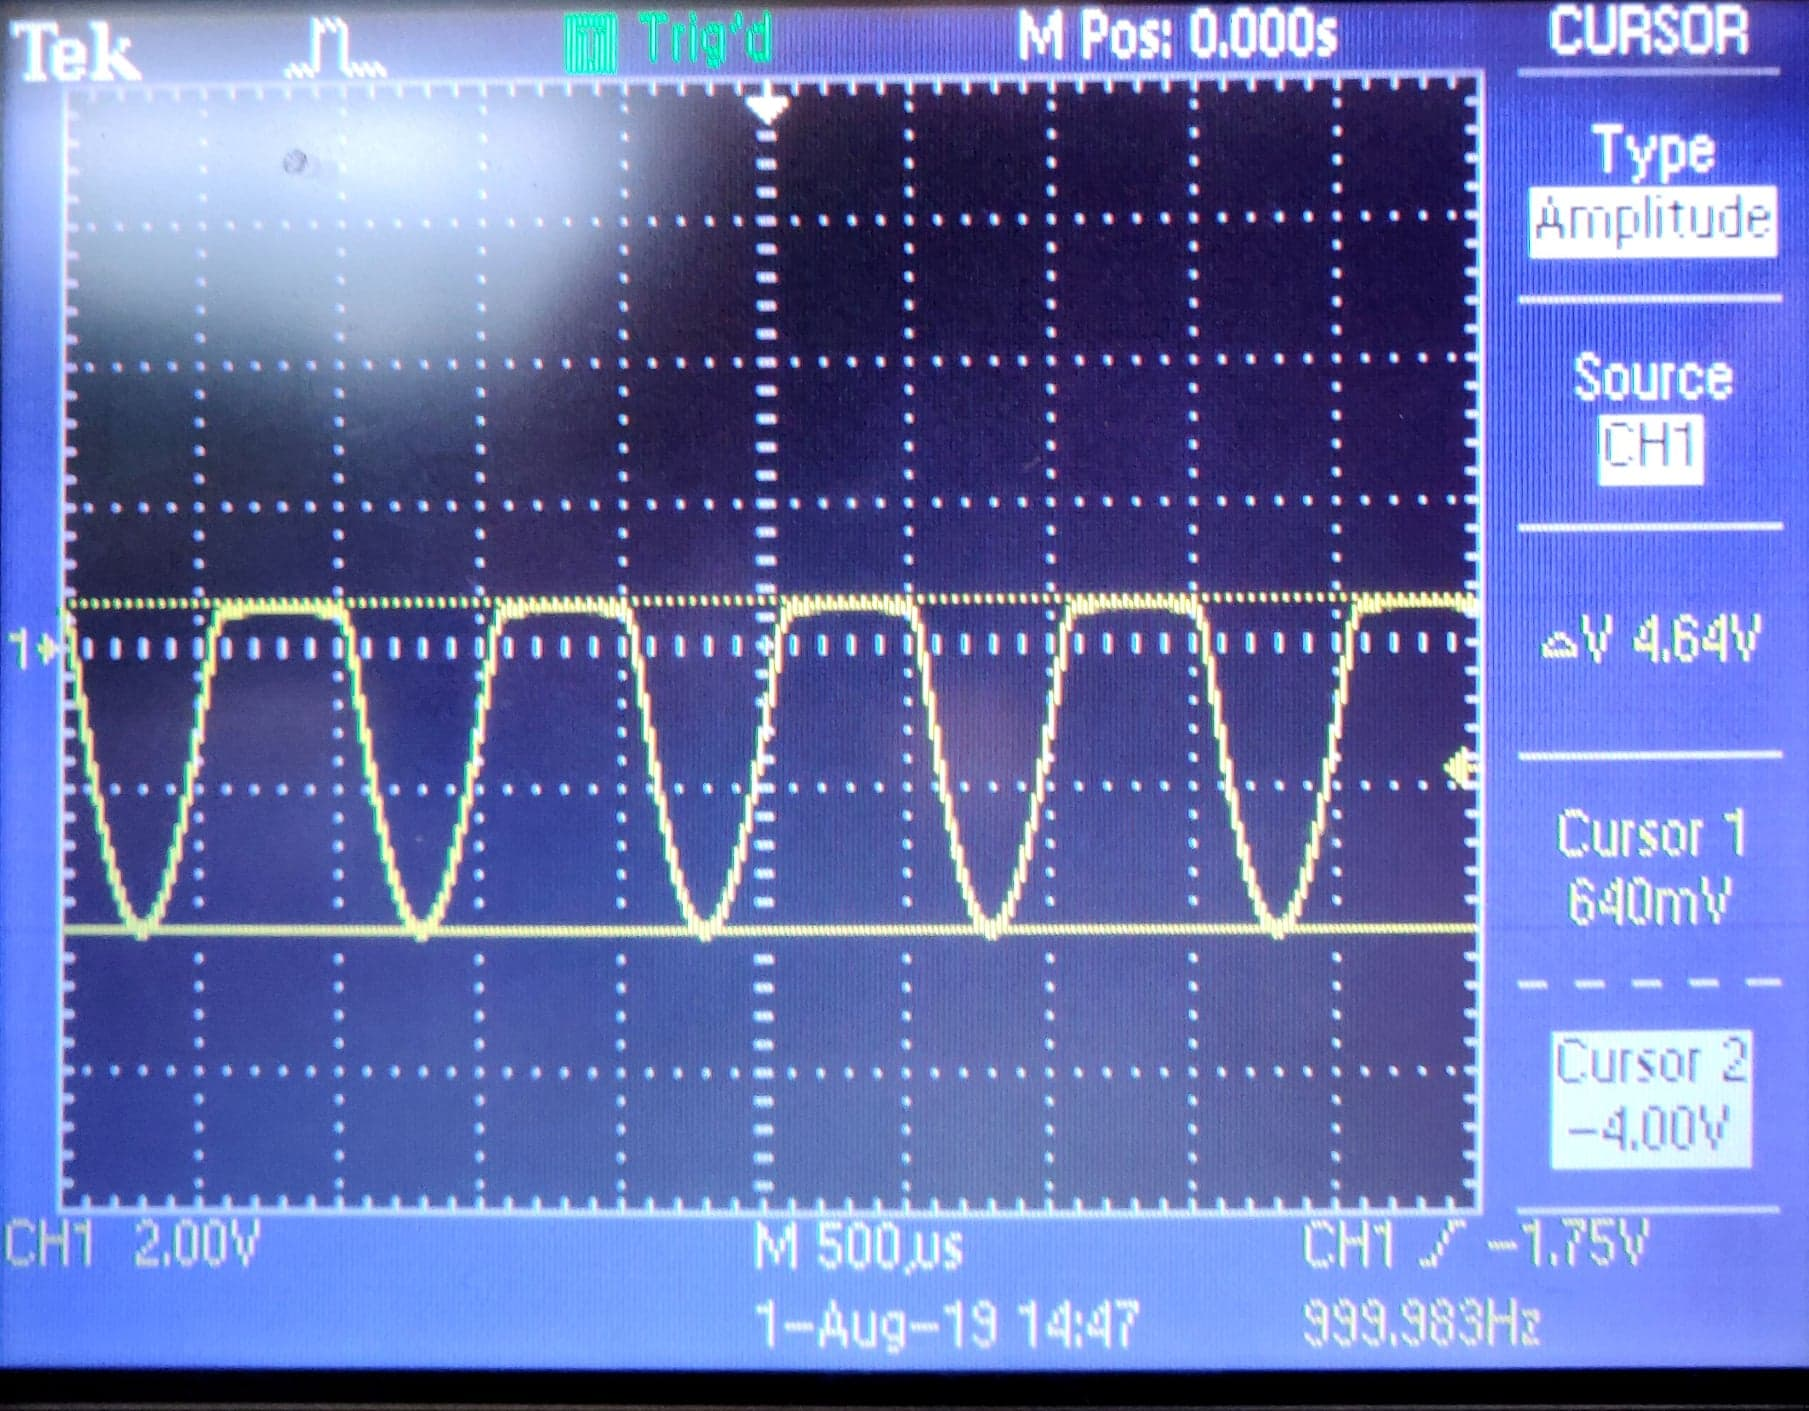
\includegraphics[width=\linewidth]{clipper.jpg}}
\caption{Diode used at a voltage clipper}
\end{figure}
In the first half of the sin wave, The diode is in forward bias. This results in a voltage drop across the diode of close to 0.7V  due to the forward activation voltage of the diode. This can be seen in figure one, the positive halves of the sin waves have been 'clipped' off, leaving a voltage of only 0.7V . In the second half the the sin wave the diode is in reverse bias. Because of this the diode can be modelled  as an open circuit, resulting in all the voltage being dropped across it.
\newpage

\begin{figure}[t]
\centering
\fbox{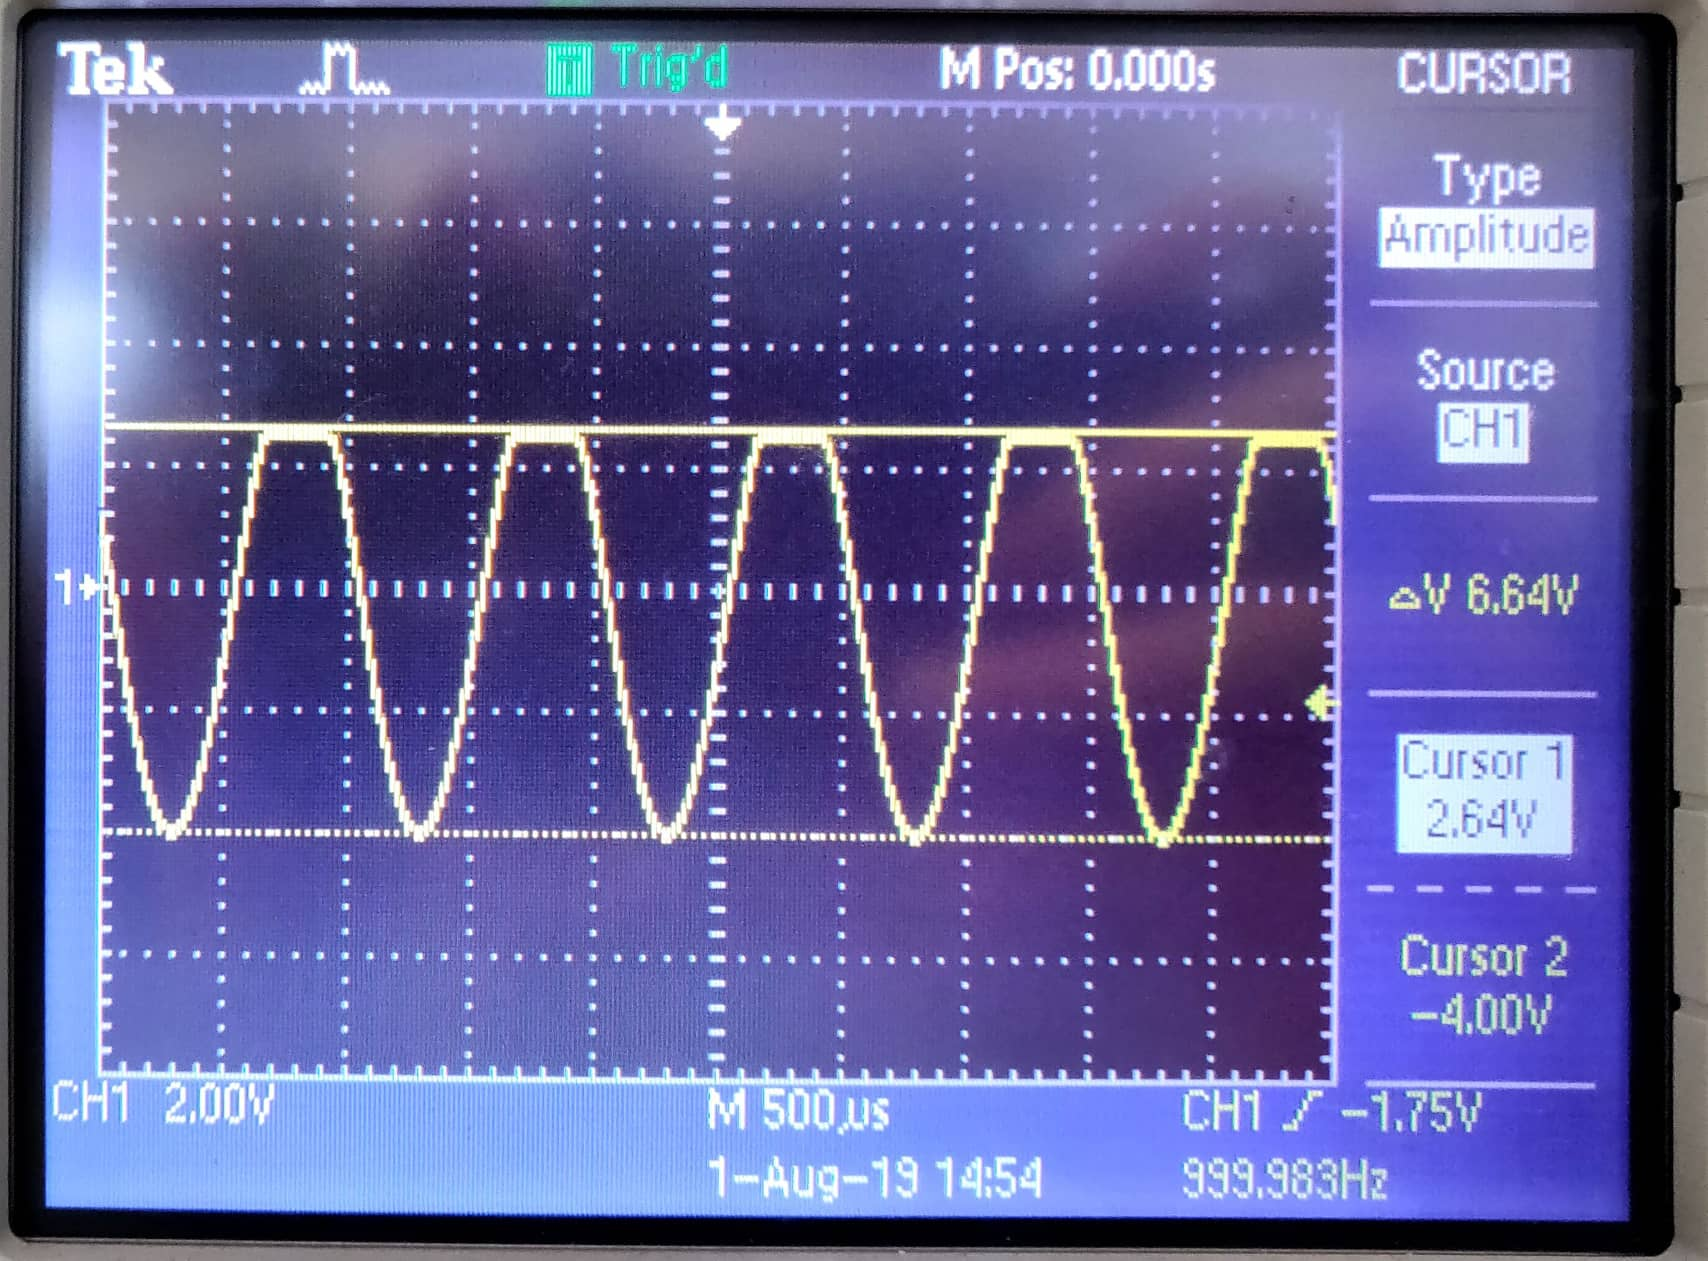
\includegraphics[width=\linewidth]{dc_inline.jpg}}
\caption{Diode used at a voltage clipper}
\end{figure}
In the first half of the sin wave, The diode is in forward bias. This results in a voltage drop across the diode of close to 0.7V  due to the forward activation voltage of the diode. However seeing as there is also a 2V DC power supply in series with the diode, there will also be a 2V drop across the power supply, giving a total voltage drop of 2.7V. This can be seen in figure two, the positive halves of the sin waves have now been 'clipped' off at a voltage of 2.6V . In the second half the the sin wave the diode is in reverse bias. Because of this the diode can be modelled  as an open circuit, resulting in all 4V being dropped across it.
\newpage

\section{Diode Clamp}
\begin{figure}[h]
\centering
\fbox{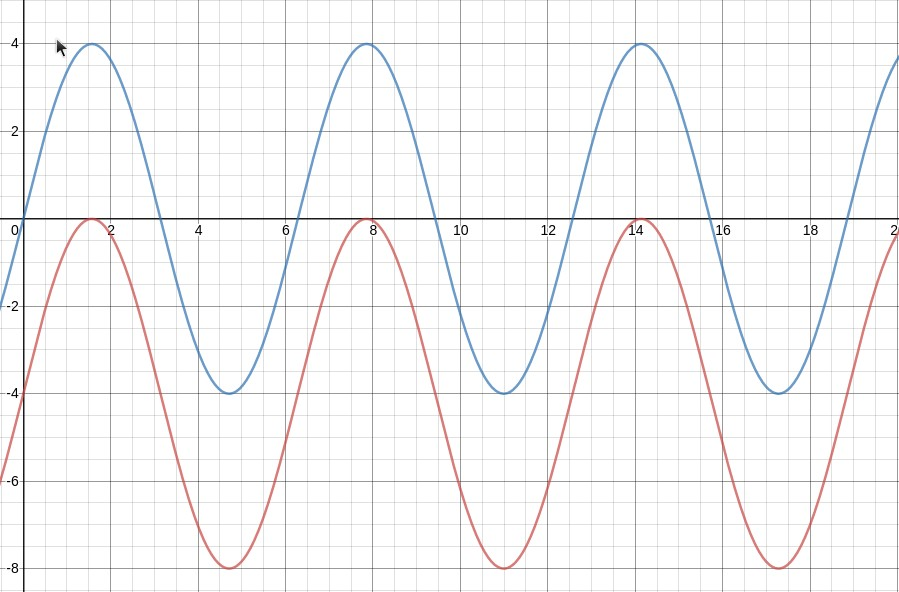
\includegraphics[width=\linewidth]{clamp.jpg}}
\caption{Diode clamp}
\end{figure}

In figure 3 we can see that the diode clamp 'clamps' the voltage to continually be negative. 	This is because when the input signal goes positive the diode will be in forward bias, allowing current to flow and charge the capacitor. However when the voltage starts to drop, the capacitor will attempt to discharge. This will place the diode in reverse bias, causing there to be a voltage drop across it. When the signal is at its lowest peak value, both the capacitor and the supply will be providing -4V, leading to the -8V drop across the diode.
\newpage

\section{Zener Diode}
\subsection{Reverse Bias Characteristic Curve}
\begin{figure}[h]
\centering
\fbox{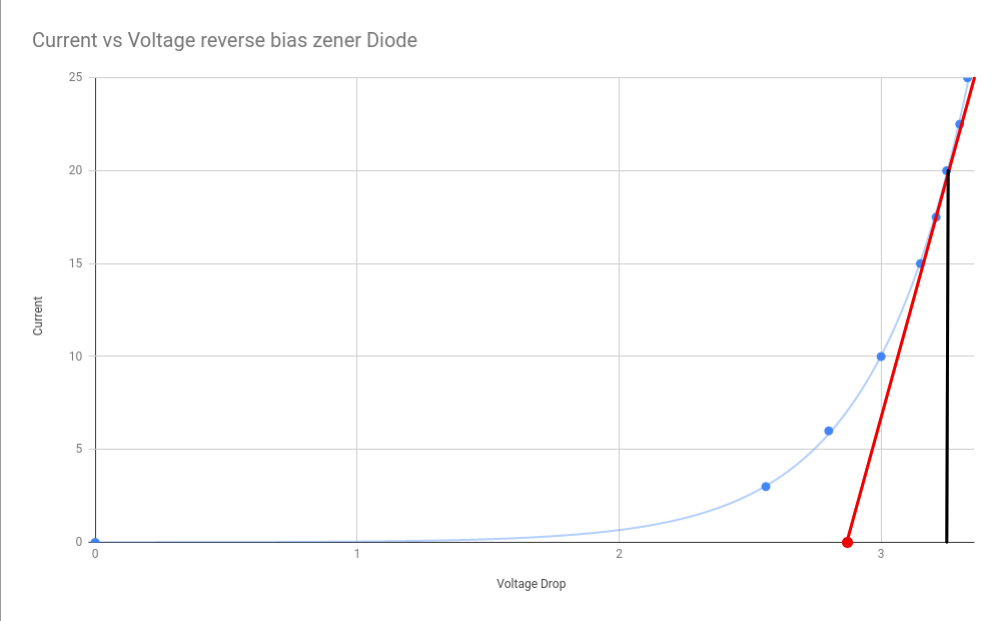
\includegraphics[width=\linewidth]{zener1.png}}
\caption{Zener diode reverse bias voltage vs current curve}
\end{figure}

Calculate $R_{z0}$ and $V_{Z0}$:\\
$V_{z0} = 2.9V$\\
$R_{z0} = \frac{\Delta V}{\Delta I}=\frac{3.25 - 2.9}{-20\times 10^{-3}} = 17.5 \Omega $

\subsection{Measured Stability ratio}
$V_s = 12V \rightarrow V_z =3.181V$\\
$V_s = 14V \rightarrow V_z =3.28V$\\
Stability ratio = $\frac{\Delta V_s}{\Delta V_z} = \frac{3.28-3.181}{14-12} = 0.049$

\subsection{Calculated Stability ratio}
Using:\\
$V_{z0} = 2.9V$\\
$R_{z0} = 17.5 \Omega $\\

Using KVO we can calculate the voltage dissipated across $R_{z0}$ at both 12V and 14V. Using this we can calculate the stability ratio.\\
$V_{s}-2.9V-R_{z0}I-470I = 0$\\
$V_s = 12V \rightarrow V_z =3.27V$\\
$V_s = 14V \rightarrow V_z =3.98V$\\
Stability ratio = $\frac{\Delta V_s}{\Delta V_z} = \frac{3.98-3.27}{14-12} = 0.036$\\

The calculated stability ratio is lower than the measured stability. I assume that this difference is due to both inaccuracies in our measurements, and also our 'guess-timations' of the value of $V_{z}$ used for the calculated stability.

\section{Additional Question}
\begin{figure}[h]
\centering
\fbox{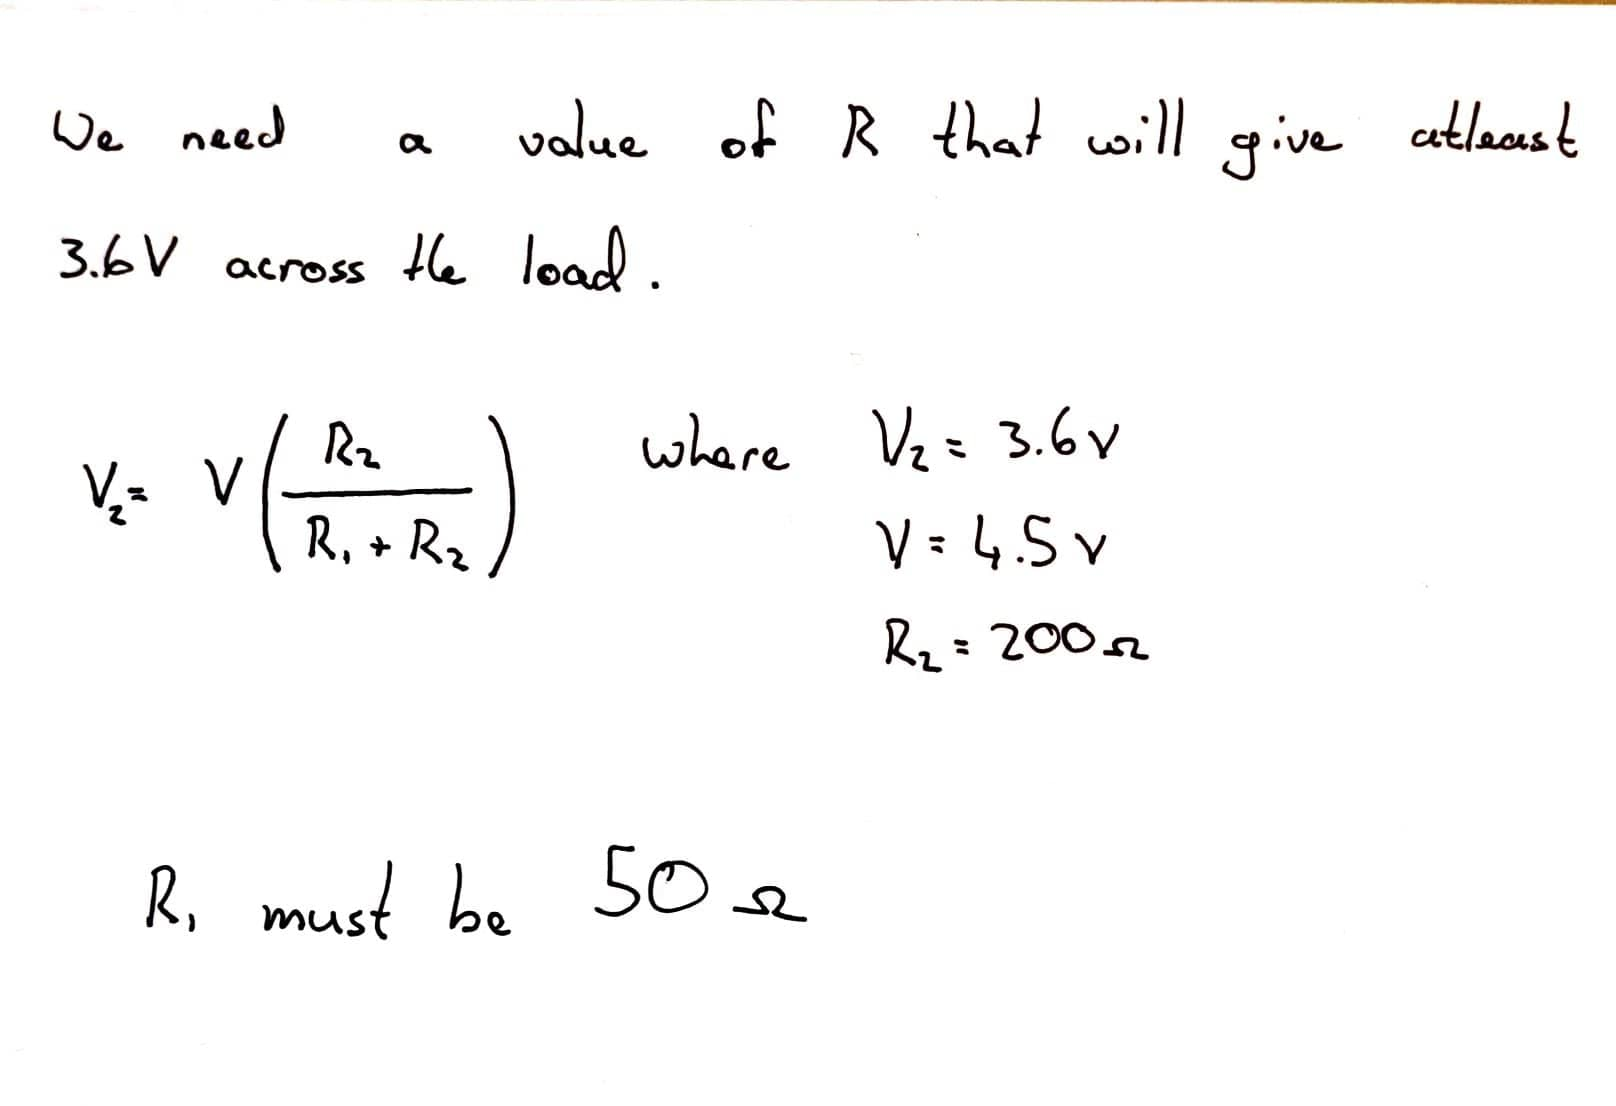
\includegraphics[width=\linewidth]{extra.jpg}}
\caption{}
\end{figure}

\end{document}
